\chapter{LCDM} % Main chapter title

\label{LCDM} % For referencing the chapter elsewhere, use \ref{Chapter1} 

%----------------------------------------------------------------------------------------

% Define some commands to keep the formatting separated from the content 
\newcommand{\keyword}[1]{\textbf{#1}}
\newcommand{\tabhead}[1]{\textbf{#1}}
\newcommand{\code}[1]{\texttt{#1}}
\newcommand{\file}[1]{\texttt{\bfseries#1}}
\newcommand{\option}[1]{\texttt{\itshape#1}}



\section{Modelo Cosmol\'ogico Est\'andar}
El modelo cosmol\'ogico mas aceptado hasta la actualidad es el conocido como \textit{Modelo Cosmol\'ogico Estandar} o $\Lambda$CDM. Este modelo utiliza la teor\'ia de la relatividad general de Einstein para la descripci\'on de la din\'amica del mismo. Se construye sobre el \textit{Principio Cosmol\'ogico}, que es la premisa de que el universo es homogeneo e is\'otropo.
Is\'otropo es un universo que luce igual en todas las direcciones, y homog\'eneo que es igual en cualquier lugar. 


Por supuesto que esto no es as\'i, ya que tenemos fluctuaciones de densidad que rompen esta supuesta homogeneidad, esto es claro por la existencia de galaxias, c\'umulos o cualquier estructura. Entonces debemos entender este principio tan solo en un sentido estad\'istico. La Isotrop\'ia se fundamenta en las observaciones del Fondo de Microondas (CMB) donde las fluctuaciones de densidad eran del orden de $10^{-5}$, es decir que el CMB es altamente is\'otropo. Si pensamos en la homogeneidad, a escalas de $\sim 200$Mpc encontramos que las propiedades estad\'isticas de conteos de galaxias son iguales. 

La m\'etrica de Robertson-Walker (RW) describe un universo bajo el principio cosmologico que se expande o contrae en funci\'on del tiempo. En coordenadas esf\'ericas, el elemento de l\'inea puede expresarse de la siguiente manera:
\begin{equation}
    ds^{2}=-dt^{2}+a^{2}(t)[\frac{dr^{2}}{1-kr^{2}}+r^{2}(d\theta^{2}+sin^{2}(\theta)d\phi^{2})]
\end{equation}{}
La variable k describe la geomegr\'ia del universo. Un valor de k=+1 corresponde a un universo con curvatura positiva, un valor de k=0 es un universo plano y un valor de k=-1 es el caso de una curvatura negativa. 

La din\'amica del universo viene dada por el factor de escala a(t). Para resolver entonces la evoluci\'on del universo uno tiene que aplicar esta m\'etrica a las ecuaciones de campo de Einstein, \textbf{HABLAR DE LAMBDA}
\begin{equation}
      R_{\mu \nu}-\frac{1}{2}Rg_{\mu \nu}-g_ {\mu \nu}\Lambda=8\pi GT_{\mu \nu}
\end{equation}{}

Para resolver estas ecuaciones, es necesario un modelo para el tensor energ\'ia-momento ($T_{\mu \nu}$). El modelo mas sencillo es el de un fluido ideal, que es caracterizado en cada punto por su densidad $\rho$ y su presi\'on p en un sistema en reposo. La forma para un tensor de estas caracter\'isticas es:
\begin{equation}
    T_ {\mu \nu}=(\rho + p)U_{\mu}U_{\nu}+pg_ {\mu \nu}
\end{equation}{}
con $U^{\mu}$ la cuadri-velocidad del fluido. Bajo l ahip\'otesis de isotrop\'ia y homogeneidad, la densidad $\rho$ y la presi\'on p solo pueden ser funciones del tiempo t. 

Ya con la m\'etrica (1.1), las ecuaciones de campo (1.2) y una forma para la materia, uno puede resolver la din\'amica de nuestro modelo cosmol\'ogico. Las ecuaciones que se obtienen son dos y son conocidas como las ecuaciones de \textit{Friedmann-Lema$\hat{i}$tre}
\begin{equation}
    H^{2}=(\frac{\dot{a}}{a})^{2}=\frac{8\pi G}{3}\rho+ \frac{\Lambda}{3}-\frac{k}{a^{2}}
\end{equation}{}
\begin{equation}
\frac{\dot{a}}{a}=-\frac{4\pi G}{3}(\rho+3p)+\frac{\Lambda}{3}    
\end{equation}
El factor H se denomica constante de Hubble y es entendida como la tasa en la que se expande el universo.

La ecuaci\'on de Friedmann relaciona la tasa en la que crece el factor de escala a(t) con el contenido de energ\'ia en el universo. Utilizando esta ecuaci\'on, podemos encontrar la densidad de energ\'ia cr\'itica $\rho_{c}$

\begin{equation}
\rho_ {c}=\frac{3H^{2}}{8\pi G}    
\end{equation}
que es la densidad de energ\'ia para la cual el universo carece de curvatura (universo plano, k=0). 

La conservaci\'on de la energ\'ia significa que 
\begin{equation}
    \nabla_{\mu}T^{\mu \nu}=0
\end{equation}{}

Donde aplicando nuestra m\'etrica de RW y el modelo de flu\'ido perfecto se obtiene una ecuaci\'on para la conservaci\'on de la energ\'ia

\begin{equation}
    \dot{\rho}+3H(\rho + p)=0
\end{equation}{}

En general, la presi\'on de un fluido se relaciona con su densidad en funci\'on de una constante $\omega$ que caracteriza a la ecuaci\'on de estado. 
\begin{equation}
    p=\omega\rho
\end{equation}{}
Los constituyentes principales del universo son radiaci\'on o materia relativista, para lo cual $\omega=\frac{1}{3}$, materia no relativista libre de presi\'on con $\omega=0$ y constante cosmol\'ogica (o energ\'ia de vac\'io) para la cual $\omega=-1$.
Para obtener la evoluci\'on de la densidad de energ\'ia de cada componente se introduce entonces la ecuaci\'on de estado en las ecuaciones de Friedmann y se encuentra que:
\begin{equation}
    \rho \sim a^{-3(1+\omega) }
\end{equation}{}



\section{Inhomogeneidades en el Universo}

El principio cosmologico, postula al universo como 'homog\'eneo e isotr\'opico'. Sobre esta hip\'otesis, se construyen algunas m\'etricas como la de Friedmann-Robertson-Walker que permiten describir el comportamiento del Universo construyendo asi modelos cosmol\'ogicos. Esta asumpci\'on de homogeneidad, se justifica solo en escalas grandes ($\sim 200 Mpc$), ya que el universo es inhomogeneo en escalas mas peque\~nas, ya que por ejemplo tenemos galaxias y c\'umulos. 

Las inhomogeneidades pueden caracterizarse en funci\'on de el contraste adimensional de densidad,
\begin{equation}
    \delta(\textbf{r},t)=\frac{\rho(\textbf{r},t) - \overline{\rho}(t)}{\overline{\rho}(t)}
    \label{ContrasteDensidad}
\end{equation}{}
donde la $\rho(\textbf{r},t)$ denota la densidad en un punto \textbf{r} a un dado tiempo t, y $\overline{\rho}(t)$ es la densidad media de materia a ese tiempo.  

De esta manera, el contraste adimencional de densidad permite caracterizar al universo en zonas \textit{subdensas}, que son aquellas donde la densidad del universo es menor que la densidad media, y en zonas \textit{sobredensas}, donde el universo adopta una densidad mayor que la densidad media de materia.



\subsection{Inestabilidades Gravitatorias}

La m\'etrica de FRW presentada en la secci\'on anterior, permite describir un universo hom\'ogeneo. La realidad tal como se menciono con anterioridad es que el universo en el que vivimos dista mucho de la homogeneidad. A\'un as\'i, el universo temprano (a alto redshift) era altamente homogeneo. Esto puede observarse en la figura \ref{CMB} donde a la izquierda tenemos una imag\'en de el fondo de microondas y a la derecha una imagen de el cat\'alogo Sloan CITA que muestra el universo local (a bajo redshift). Las perturbaciones de densidad de el universo hoy, son del orden de  $\delta \sim 10^{3}$ mientras que el CMB presenta perturbaciones de $\delta \sim 10^{-5}$ lo cual es practicamente un universo homog\'eneo.

 

\begin{figure}[h]
\centering
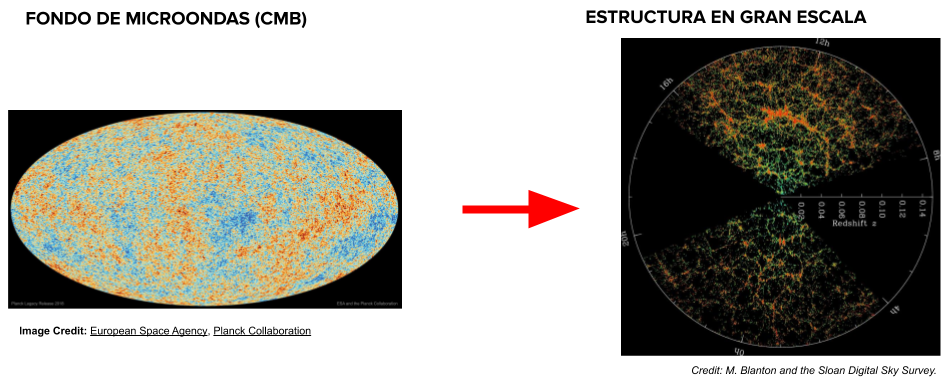
\includegraphics[width=10cm]{Figures/SeminarioII_agustin_rodriguez.png}
\decoRule
\caption[CMB]{Izquierda: Fondo de Microondas ($z\sim 3000$)}, imagen tomada de la colaboraci\'on Planck. Derecha: Universo cercano $(z\sim 0)$ de el cat\'alogo SDSS.
\label{CMB}
\end{figure}

La pregunta que surge es como hizo entonces el universo para pasar de ser altamente homogeneo a convertirse en un universo altamente inhomogeneo, dando lugar de esta manera a las galaxias y sistemas de estas. Y la respuesta a esta pregunta viene dada por las siguientes ecuaciones que describen la evolucion de las perturbaciones gravitatorias que, junto a otros procesos hidrodin\'amicos, generaron las estructuras que hoy en d\'ia conocemos como galaxias o c\'umulos. 

\begin{equation}
    \frac{\partial{\rho}}{\partial{t}}+\frac{3\dot{a}}{a}\rho+\frac{1}{a}\nabla.(\rho\textbf{u})=0
    \label{continuidad}
\end{equation}{}

\begin{equation}
    \frac{\partial{u}}{\partial{t}}+\frac{\textbf{u}.\nabla}{a}\textbf{u}+\frac{\dot{a}}{a}\textbf{u}=-\frac{1}{\overline{\rho}a}\nabla{P}-\frac{1}{a}\nabla{\Phi}
    \label{euler}
\end{equation}{}

\begin{equation}
    \nabla^{2}\Phi(\textbf{x},t)=4\pi Ga^{2}(t)\overline{\rho}\delta(\textbf{x},t)
    \label{poisson}
\end{equation}{}

\begin{equation}
    p=\omega \rho
    \label{estado}
\end{equation}{}

La ecuacion \ref{continuidad} es conocidad como la ecuaci\'on de continuidad, que expresa simplemente la conservaci\'on de la masa. La segunda ecuaci\'on, \ref{euler} es conocidad como ecuaci\'on de la conservaci\'on del momento o ecuaci\'on de Euler. Esta ecuaci\'on vectorial detalla el movimiento de las particulas, en el lado derecho tenemos un t\'ermino que responde a el potencial gravitacional $(\Fi$) y un termino que responde a la presi\'on ($P$). Estos gradientes son llamados \textit{terminos fuentes} de la ecuaci\'on de Euler. Si bien en esta formulacion solo se incluyen dos t\'erminos fuentes, pueden incluirse otras fuentes de fuerzas tales como campoes electromagn\'eticos.. etc. La ecuaci\'on \ref{Poisson} relaciona el potencial gravitacional generado por una distribuci\'on inhomogenea de materia ($\delta$) que depende del tiempo y de la posici\'on. Finalmente la ecuaci\'on \ref{estado} me relaciona a la presi\'on (p) con la densidad de materia ($\rho$) donde a diferentes tipos de materia (gas, materia oscura, etc) corresponden diferentes constantes $\omega$. 

%Para estudios cosmologicos es conveniente reescribir las ecuaciones \ref{continuidad} y \ref{euler} en t\'erminos de coordenadas en expansi\'on y en funci\'on de el contraste adimencional de densidad $\delta$ CITA PEEBLES, quedando entonces:

%\begin{equation}
%    \frac{\partial v}{\partial t} + \frac{1}{a}(\textbf{v} \cdot \nabla)\textbf{v} + \frac{\dot{a}}{a}\textbf{v}=-\frac{1}{\rho a}\nabla p - \frac{1}{a}\fi
%\end{equation}{}
%\begin{equation}
%    \frac{\partial \delta}{\partial t}+ \frac{1}{a}\nabla \cdot (1 + \delta )\textbf{v}=0
%\end{equation}{}



Como puede verse en el set de ecuaciones presentado, este constituye un sistema acoplado y altamente no lineal. La resoluci\'on entonces de estas ecuaciones para el estudio de la evoluci\'on de las perturbaciones de densidad es de gran dificultad y solo puede resolverse an\'aliticamente para casos que requieren un alto grado de simplificaciones y aproximaci\'on, para lo demas, es menester el uso de otras herramientas como las simulaciones num\'ericas, sobre las que no explayaremos en la siguiente secci\'on. 



\subsection{Teor\'ia de perturbaciones lineales}
\label{PerturbacionesLineales}

Un resultado an\'alitico para las ecuaciones que describen la evoluci\'on de las pertubaciones de densidad (\ref{continuidad},\ref{euler},\ref{poisson}) es posible al realizar un aproximaci\'on lineal, v\'alida para casos restringidos pero de suma importancia, como veremos m\'as adelante.


Consideraremos peque\~nas pertubaciones de densidad sobre un universo homog\'eneo ($\delta \ll 1 $). Para trabajar con las ecuaciones \ref{continuidad} \ref{euler} primero las escribiremos en t\'erminos de el contraste $\delta$ y luego consideraremos t\'erminos de primer orden en $\delta$ y \textbf{u}. De esta manera, manipulando algebraicamente las ecuaciones obtenemos las siguientes relaciones para la evoluci\'on del contraste de densidad \citep{ElPeebles}
\begin{equation}
 \frac{\partial^{2}\delta}{\partial t ^{2}}+ \frac{2 \dot{a}}{a}\frac{\partial \delta}{\partial t}=4\pi G   \overline{\rho}\delta 
 \label{EcuacionDeltaAproximacion}
\end{equation}

\begin{equation}
    \frac{\partial ^{2}{\delta}}{\partial t ^{2}}+ \frac{1}{a}\nabla \cdot \textbf{u}= 0
\end{equation}{}

Queda expl\'ito que la soluci\'on para el contraste $\delta$ no depende de la posici\'on (al menos para la aproximaci\'on lineal), por lo que las soluciones seran de la forma 
\begin{equation}
    \delta({\textbf{x},t})=D(t)S(\textbf{x})
\end{equation}{}

Bajo esta forma funcional, del hecho de que el contraste no tiene una dependencia espacial, se puede realizar una expansi\'on en el espacio de Fourier de las frecuencias espaciales donde el contraste de densidad $\delta$ adoptar\'ia la siguiente forma:

\begin{equation}
    \delta(\textbf{x})=\sum_{i=0}^{\infty} \hat{\delta}(\textbf{k}) e^{-i\textbf{k}\cdot \textbf{x}}
    \label{seriefourier}
\end{equation}{}

De modo que vemos que podemos representar al universo como una superposici\'on de ondas de diferentes fases, cuya amplitud viene dada por un espectro de potencias.
\begin{equation}
    P(k)=<\mid \hat{\delta}(k) \mid ^{2}>
\end{equation}{}



\section{Vac\'ios en la literatura}

La figura \ref{SDSS} presenta la distribuci\'on de galaxias del universo cercano obtenida por el proyecto \textit{Sloan Digital Sky Server}, conocido como SDSS. \textcolor{red}{CITA}. Pueden aprecirse como las regiones sobredensas del universo rodean zonas subdensas, conocidas como \textit{cosmic \textbf{voids}}. Estas regiones, pensadas taxonomicamente como una componente de la estructura en gran escala del universo, constituyen la mayor parte del contenido del universo \citep{Sheth2004}.

T\'ipicamente alcanzan contrastes de densidad de $\delta\simeq$-0.9. No existe un consenso en cuanto a la forma de estos, aunque la tendencia general es que se tornen estructuras esf\'ericas \citep{Sheth2004}. Lo mas facil es identificarlos con formas esf\'ericas, aunque tambi\'en pueden adoptarse otros criterios para esto. 

Existen diversos estudios realizados con c\'atalogos de diferentes relevamientos sobre las propiedades de las galaxias que habitan estos entornos subdensos. Estos carecen de galaxias brillantes y su estructura interna es trazada fundamentalmente por galaxias d\'ebiles \citep{Alpaslan2014}. En general, la din\'amica interna de los vac\'ios es expansiva \cite{Sheth2004} por lo que las galaxias dentro de estos ambientes siente una constante de hubble mayor. De esta manera la formaci\'on de estructuras dentro de los vac\'ios es mas lenta que en otro ambientes \citep{Kreckel2016} ? \cite{Tomita2000} . Esto otorga a las galaxias en voids propiedades muy caracteristicas. \citep{Ceccarelli2008} encuentra que estas son azules y con tasas altas de formaci\'on estelar. De modo que existe una modulaci\'on de la gran escala en estas propiedades astrof\'isicas que va mas all\'a de el entorno local. 




\begin{figure}
    \centering
    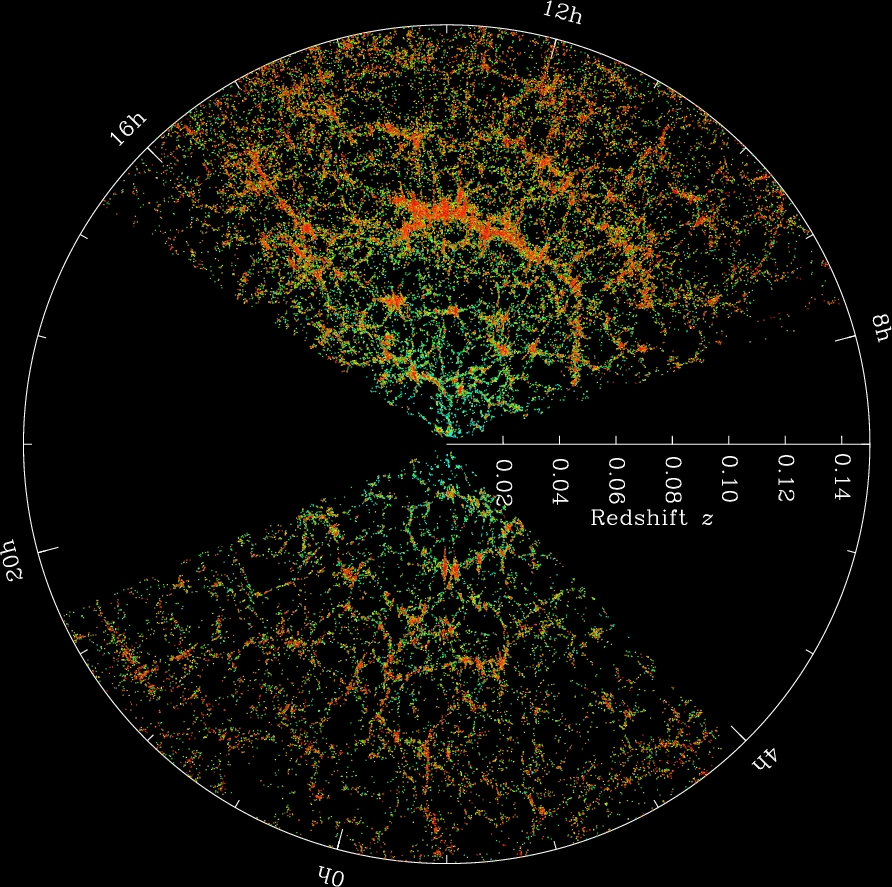
\includegraphics[width=10cm]{Figures/orangepie.jpg}
    \caption{Caption}
    \label{SDSS}
\end{figure}{}

%\section{Simulaciones Num\'ericas}
%Segun el paradigma del universo $\Lambda CDM$, la densidad de materia en el universo esta dominada por la materia oscura. Por lo cual, la din\'amica general del universo esta dominada por la din\'amica de la materia oscura, y la materia bari\'onica acompaña esta din\'amica, introduciendo efectos que, al menos en un principio, se espera que sean \textit{secundarios}. 
%De modo que una descripci\'on detallada de lo que le suceda a , por ejemplo, una galaxia requerir\'a de simular las interacciones de N-cuerpos de materia oscura. Si quisiera representarse cada estrella en una galaxia con una particula, esto requeria de $\sim 10^{10}$particulas, y estos n\'umeros son imposibles de simular, por lo cual, las t\'ecnias actuales requieren de algunas simplificaciones de los problemas. En particular, se discretiza las distribucion de materia considerando un n\'umero de particulas mucho menor al real. 

%\subsection{Ecuaci\'on de Bolzmann}

%La aproximaci\'on utilizada para resolver los problemas de N-cuerpos, requiere considerar a las particulas en un sentido estad\'istico. Cada part\'icula simulada representa entonces una poblaci\'on de part\'iculas f\'isicas (de estrellas, gas, materia oscura, etc.) con propiedades f\'isicas similares, es decir, casi posiciones identicas o velocidades. La evoluci\'on de estos ensambles de part\'iculas es gobernada entonces por la mec\'anica estad\'istica. 

%Podemos pensar al universo entonces como un \textit{fluido} descripto por las ecuaciones  de la hidrodin\'amica. El n\'umero de particulas dN, con posiciones entre \textbf{x + dx}, velocidades \textbf{u + du} en un tiempo t es entonces
%\begin{equation}
%    dN=f(\textbf{x}, \textbf{u}, t)\textbf{dx}\textbf{du}
%\end{equation}{}
%Un elemento de volumen que contenga un n\'umero suficientemente grande de part\'iculas podra ser tratado estad\'isticamente. Suponemos sus posiciones entre \textbf{x+dx} y con velocidades \textbf{u+du}, y consideremos un campo de fuerza \textbf{F} que no cambia apreciablemente con distancias comparables a la distancia media entre part\'iculas. Sea \textbf{q} el momento, tal que \textbf{q}=m\textbf{u}, entonces se encuentra que
%\begin{equation}
%    \frac{\partial{f}}{\partial{t}}+u_{i}\frac{\partial{f}}{\partial{}x_{i}}+F_{i}\frac{\partial{f}}{\partial{u_{i}}}=[\frac{\partial{f}}{\partial{t}}]_{col}
%\end{equation}{}
%Esta es conocida como la \textit{Ecuaci\'on de Boltzmann} y describe la evoluci\'on de una funci\'on distribuci\'on en el espacio de seis dimensiones (\textbf{x}.\textbf{u}) llamado espacio de fases.  Expresa el hecho de que el cambio en el n\'umero de particulas en un elemento de volumen del espacio de fases es igual a el n\'umero de particulas que entran o dejan el elemento. 



%\subsection{Condiciones Iniciales}

%\subsection{Metodos de integraci\'on}

%\subsection{SPH}

